\documentclass[12pt,oneside,reqno]{amsart}
\usepackage[left=3cm,right=3cm,top=3cm,bottom=2cm]{geometry} % page settings
\usepackage{amsmath} % provides many mathematical environments & tools
\usepackage{amssymb}
\usepackage{natded}
\usepackage{booktabs}
\usepackage{graphicx}
\usepackage{hyperref}

\begin{document}
\setlength{\parindent}{6pt}
\def\code#1{\texttt{#1}} %Code looking
\def\ra{\rightarrow{}} %Short for right arrow
%\def\proof{\proofline{\amsmath}{}} %Short for right arrow
\newcommand{\itab}[1]{\hspace{0em}\rlap{#1}}
\newcommand{\tab}[1]{\hspace{.2\textwidth}\rlap{#1}}
\newcommand\deff{\mathrel{\stackrel{\makebox[0pt]{\mbox{\normalfont\tiny def}}}{=}}}
\raggedbottom

\title{Josefin Ondrus\\ondrus@student.chalmers.se}
\author{DAT060 Exercise week 6}
\date{\today}
\maketitle

%************************Q1
\textbf{Problem 1}\\
%*************************
\textbf{a}\\

\textbf{b}\\

%************************Q2
\textbf{Problem 2}\\
%*************************
Drawing the graph we get: 
	\begin{figure}[h]
      	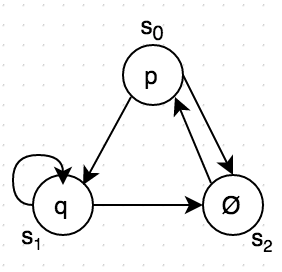
\includegraphics[scale=0.7]{prob2}
	\end{figure}\\
\textbf{a} is satisfied on all paths in M\\
This because no matter what state we start from ether $\neg p$ or $\neg q$ will hold. There is only one path where we do not pass $\emptyset$ and that is $s_1 ->s_1->s_1 ->...$ where $\neg q$ hold, making the LTL-formula satisfied (assuming $\neg p, \neg q \text{ holds in } \emptyset$).\\\\
\textbf{b} is satisfied on all paths in M\\
$\neg p$ keeps happening in all paths. Since there is only one state where $p$ holds and this is in $s_0$, we know that this LTL-formula is satisfied in some future state for all paths. This because there is no path with only $s_0$ (i.e. $s_0->s_0->s_0->...$).\\\\
\textbf{c} is satisfied on all paths in M\\
There is only one path where $GFp$ is false and that is in path $s_1->s_1->s_1->...$. If we check the state on the left hand side of the cause (which needs to be true in order for the formula to fail in this M) we see that the left hand side is false (because $q$ holds) and therefor there is no path not satisfying this LTL-formula.\\\\
%************************Q2
\textbf{Problem 3}\\
%*************************
\textbf{a} These CTL-formula are not equivalent\\
Given the following transition system we can see that the left statement holds but not the right. (The path breaking the right statement is $s_0->s_1->s_0->s_1...$)
	\begin{figure}[h]
      	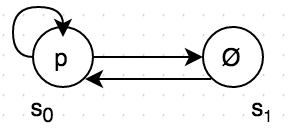
\includegraphics[scale=0.7]{prob3a}
	\end{figure}\\\\
\textbf{b} These CTL-formula are not equivalent\\
Given the following transition system we can see that the left statement holds but not the right. There is no state in this transition system that fulfills the right statement but all paths fulfills the left.
	\begin{figure}[h]
      	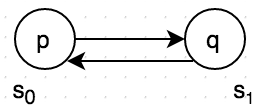
\includegraphics[scale=0.7]{prob3b}
	\end{figure}\\\\
\textbf{c} These CTL-formula are equivalent\\\\
Explaining there two formulas in text make it obvious that they need to be equivalent. The left formula states that $p \land q$ does not hold in all paths. The right formula claims that $\neg p$ or $\neg q$ will happens sometime in the future in at least one path. If $p \land q$ does not hold in all paths there must exists at least one path where $\neg p$ or $\neg q$ will happens at least one along the path.\\\\
Or if you prefer:
We know $\neg AG(p \land q) = EF\neg(p \land q)$.\\
Through De Morgan's we can rewrite the formula as $\neg AG(p\land q) = EF(\neg p \lor \neg q)$\\
and by the equivalence $EF(\varphi_1 \lor \varphi_2)=EF\varphi_1 \lor EF\varphi_2$\\ we can state that $\neg AG(p\land q) = EF\neg p\lor EF\neg q$\\
Which is the equivalence that should be proven.\\\\
\textbf{d} These CTL-formula are not equivalent\\
Since $\varphi_1 U \varphi_2$ demands that $\varphi_2$ does hold in some future state; the right formula demands that both $q$ and $r$ holds in some future state in all paths. However, the left formula demands that $A[q U r]$ and $r$ holds in some future state for all paths. And since $A[q U r]$ is fulfilled if $r$ holds where we start the path (since the present is included in the future). We can prove that the formulas are not equivalent with the transition system below where the left formula holds but not the right (since $q$ never holds in some future). 
	\begin{figure}[h]
      	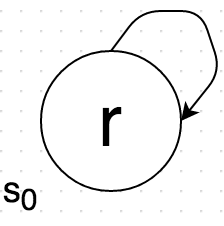
\includegraphics[scale=0.7]{prob3d}
	\end{figure}\\\\
\end{document}